\todo[color=red]{move this to later, probably before depth interfacing}
Or more interestingly other sensors, such as depth or force sensors on robot hands or grippers (\todo{inspired by the MILES paper, talk about this}). This relates back to the idea of human perception. To learn new tasks, we use all kinds of feedback from the environment that is reactive on our actions. Therefore, it is important to study shortcomings of individual sensors with respect to others to understand how policies with limited access to sensors can be made to overcome such challenges without necessarily adding more `observability' to a workspace, which is the main problem we are trying to address with later active systems.\todo[color=blue]{reread and shorten if needed}


\section{Depth Interfacing}
Another area of important research, before relating all this back to active vision, is figuring out distance. Depth interfacing is an important part of perception. Continuing from the drawn parallels to humans, we place object in our fields of vision by our two eyes. Stereo-vision, allows us to process two slightly different poses of a target object to reinforce our understanding of where that object is in the environment around us. Other information such as lighting (shadows) may unconsciously help us as well. However, the main takeaway is that understanding distance to an object goes a long way in firstly understanding how to approach an object.

The few ways to achieve this in robotics and RLBench specifically is either to use two cameras (with a known distance between the two cameras to adjust poses with known intrinsics). However, RGB cameras are not the only things we have access to in this system. We also we have access to a depth sensor -and the point cloud information which is derived using this information.

This is because, as I hinted earlier in the background section, the main idea of active vision is to be able to use minimal amounts of viewpoints and make the most out of these. In this scenario, I want to see if it can be justified to use the wrist camera accompanied by the wrist depth sensor to replace any other cameras we might have around the workspace. Paving the way to the next section in proposing active vision policies that act solely on information from a repositionable sensor (be that rgb, depth or any other).

So, I want to see whether depth data adds meaningful information that we can justify not using external scene cameras in favour of a wrist camera and a wrist depth sensor.

\section{Grasping with Varying Depths}
I want to investigate how the an agent might react to different sized targets that might be placed at different distances from the gripper.

\subsection{Task Design}
The experiment that makes sense in this case is a grasping task. Because unlike the reaching tasks from earlier, the robot will need slightly more precision in executing its grasp and actually grabbing the target.

As the task performer needs to figure out where an object is before attempting to grab it. So, I created a modified version of the simple grasping task where the target object's distance and scale can be externally varied to observe the behaviours of agents in a controlled manner.\todo[color=green]{talk about delegating the task creating and param passing as wellas the tasks in appendix and link here}

\begin{figure}[htpb] % htpb allows all placement
  \begin{subfigure}{0.4\linewidth}
    \centering
    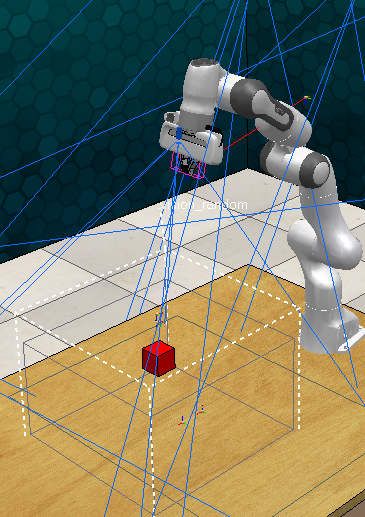
\includegraphics[width=0.7\linewidth]{assets/depth-interfacing/normal-size-grasp.png}
    \caption{Normal Sized Cube}\label{subfig:normal-grasp}
  \end{subfigure}
  \hfill
  \begin{subfigure}{0.4\linewidth}
    \centering
    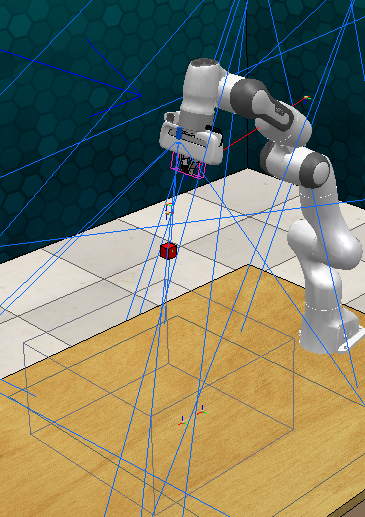
\includegraphics[width=0.7\linewidth]{assets/depth-interfacing/smaller-grasp.png}
    \caption{Small Sized Cube}\label{subfig:small-grasp}
  \end{subfigure}
  \begin{subfigure}{0.4\linewidth}
    \centering
    
\includegraphics[width=0.7\linewidth]{assets/depth-interfacing/normal-size-wrist.png}
    \caption{Wrist RGB from Normal Sized Task}\label{subfig:normal-rgb}
  \end{subfigure}
  \hfill
  \begin{subfigure}{0.4\linewidth}
    \centering
    
\includegraphics[width=0.7\linewidth]{assets/depth-interfacing/smaller-wrist.png}
    \caption{Wrist RGB from Smaller Sized Task}\label{subfig:small-rgb}
  \end{subfigure}
  \caption{Visualisation of the Depth Interfacing experiment task}\label{fig:di-task}
\end{figure}

This is the general setup I am planning on using to evaluate the depth sensor versus a stereo or any multi-view setup. 
\todo{put the other graphics already in the thing}

As we can see here, in these very different reaching scenarios \todo{ref the figure} the wrist inputs are the same, or very similar, due to the different placements of the targets. However, if we look at the stereo setup, for example \todo{ref the l and r cams}, the objects can be distinguished. Or if we were to have a stereo wrist RGB setup \todo[color=red]{not sure if this is possible I hate changing anything in RLBench, maybe mention trying if i have the time to} or \todo{link other figure} the depth features might be able to help distinguish these 2 views.
\missingfigure{add the left and right shoulder cams here 2 by 1 figure, of the above task}
\missingfigure{add differnt depth outputs from the above task, 2 by 1 figure}

\section{Creating an Appropriate Policy}
The policy for grasping needed slight modifications compared to the simpler reaching task. Along with understanding what is being seen for movement of the joints, we also needed a mechanism for sending a grasping signal for the robot. The previous policy would regress the entire 6DoF along with the final \emph{float} that controls the gripper. This was not sufficient for this task. Firstly, there weren't many frames the gripper is signaled to be closed, as the gripping happens at the end of the task, comparatively less observations where the gripper is closed; means that there is an inherent imbalance in our dataset. If we were to treat \textbf{CLOSED} and \textbf{OPEN} as binary labels; which they are as RLBench takes a \emph{float} $\in \left[0, 1\right]$ and thresholds at $ > 0.9$ to check if it should be open. Therefore, regressing the entire action with the gripper bit makes it extremely uncertain and mostly skew towards staying open. 

To adjust for this I first tried to do binary classification with weighting the samples to counteract this, which was not fruitful just due to the overall dataset size being small as well. So, going back to regression, I decided to add Cross Entropy Loss and with a gripper prediction head just predict the gripper action from the extracted camera features, then add this as a part of the overall loss with a weighting \todo{add loss in math notation with lambda gripper}. This meant that the gripper action is separately tunable to the movement action. This makes inherent sense as the movement decisions should never affect the gripper. The information flow is camera to movement and gripper action separately \todo{small flowchart to show cam  move, cam gripper action} 


\subsubsection{Incorporating the Depth Camera}
probably cant just fuse with the rgb, might need a new conv for this then merger header

\todo{conclude depth here and move onto combination experiments}

